\clearpage
\section{Approksimering av distributed systems}\label{sec:distributed}
Et distributed system er et anisotropisk system med hensyn på intensive variabler. Det vil si at i et volum er, for eksempel, temperaturen avhengig av posisjonen i volumet. Som prosessingeniører må vi ofte lage en modell for denne anisotropiske oppførselen. Mange av disse modellene kreverer mye prosessorkraft og noen er rett og slett umulig å løse analytisk. I slike tilfelles må vi sette opp en approksimasjon for modellen. Her har vi flere metoder og vi starter med den enkleste som har fått kallenavnet $"$Sliced Salami$"$.

\subsection{Sliced Salami method}
Sliced salami metoden er en måte å dele et distributed system inn i flere lumped systems. På den måten trenger vi ikke en modell for transporten gjennom det distributed systemet, men trenger istedet transporten mellom de mindre kontrollvolumene. Som du ser i \cref{fig:Sliced_salami} er analogien at man tar salamien (Distributed system) og kutter det opp i flere mindre biter (lumped systems). Hver av disse systemene har egenskaper som tilsvarer posisjoner i det distributede systemet. 

\begin{figure}[H]
    \centering
    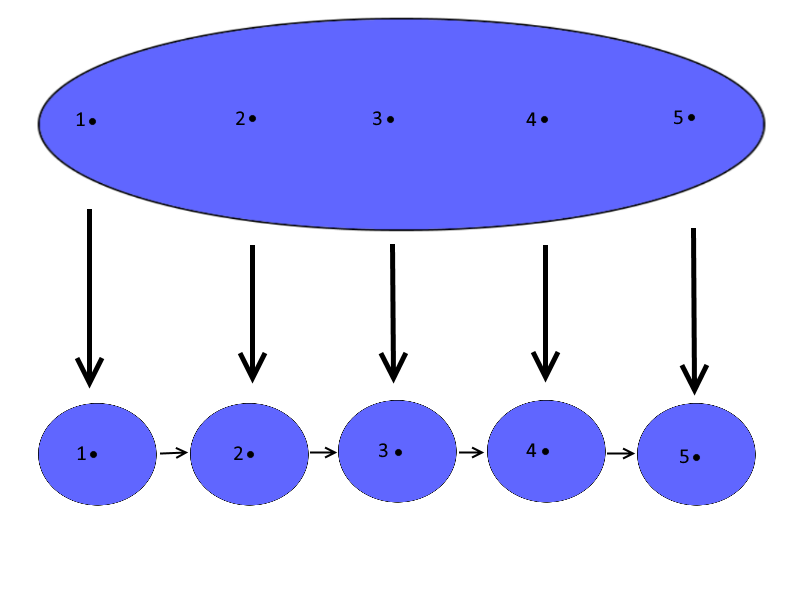
\includegraphics[scale=0.4]{Figures/sliced_salami_method.png}
    \caption{Visualisering av Sliced Salami Method. Et Distributed system deles opp i lumped systems.}
    \label{fig:Sliced_salami}
\end{figure}

\subsection{Numerisk approksimasjon}\label{sec:numerisk_approksimasjon}
En annen metode trekker deg tilbake til vårsemesteret og faget Matte 4N. Vi starter med å dele systemet vårt inn i et grid med punkter som spenner over rommet i de retninger hvor de intensive variablene varierer. 
\begin{figure}[H]
    \centering
    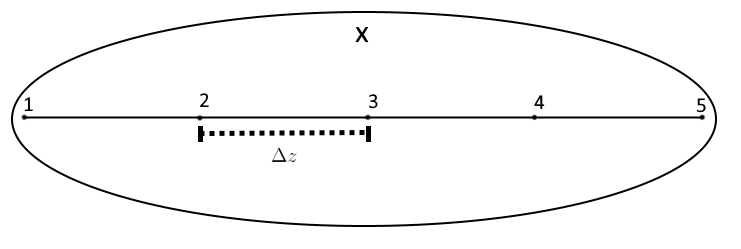
\includegraphics[scale=0.5]{Figures/Distributed_discret.png}
    \caption{Distributed system med intensiv variabel $x$, delt opp i et 1-dimensjonalt grid med 5 punkter og steglengde $\Delta z$.}
    \label{fig:distributed_numerisk}
\end{figure}

I \cref{fig:distributed_numerisk} ser vi at variabelen $x$ endres fra posisjon 1 til posisjon 5. Vi har mange måter å approksimere endringen av $x$ langs $z$ og de fleste bygger på en Taylor utvidelse. Uten å bruke tid på å argumentere for hvorfor dette fungerer setter vi opp en Taylor utvidelse som evaluerer $i+1$ fra posisjon $i$ med lengde $\Delta z$:

\begin{align}
    x_{i+1} = x_i + \frac{dx_i}{dz}\Delta z + \frac{1}{2!}\frac{d^2x_i}{dz^2}(\Delta z)^2 + \frac{1}{3!}\frac{d^3x_i}{dz^3}(\Delta z)^3 + \dots
\end{align}

Litt skummel formel, men likevel nyttig å kunne (pst, dette er fra Matte 1 om du ikke husker). Som oftest i numeriske approksimasjoner benytter vi oss kun av de to første leddene:
\begin{align}
    x_{i+1} &\approx x_i + \frac{dx_i}{dz}\Delta z\\
    &\downarrow \\
    \frac{dx_i}{dz} &\approx \frac{x_{i+1}-x_i}{\Delta z}
\end{align}
Nå som vi har en approksimering for $\frac{dx_i}{dz}$ kan vi sette denne inn for ukjente differensialer, e.g. transportligninger. Approksimeringen vi har i ligningen over er navngitt \textit{Forward method} og er forhåndsvis enkel å bruke. Under har vi lagt fram de vi mener er viktigste numeriske metodene for approksimering av differensialer. 

\begin{equation}
    \begin{split}
    \label{eq:numerical_approx}        
    \text{Forward method: }\frac{dx}{dz}\Big|_i &\approx \frac{x_{i+1}-x_i}{\Delta z} \\
    \text{Central method 1th order: }\frac{dx}{dz}\Big|_i &\approx \frac{x_{i+1}-x_{i-1}}{2\Delta z}\\
    \text{Central method 2th order: }\frac{d^2x}{dz^2}\Big|_i &\approx \frac{x_{i-1}-2x_i+x_{i+1}}{(\Delta z)^2}
    \end{split}
\end{equation}
    

\subsection{Numeriske skjemaer}
Med den numeriske approksimasjonen kan vi substituere ligningene fra (\ref{eq:numerical_approx}) inn i en differensial ligning slik at vi kan benytte oss av programmering til å løse problemet. Uten å bruke for mye tid og krefter på å forklare dette trekker vi fram et enkelt eksempel.

\subsubsection{Eksempel: Euler's method}

\begin{equation}
    \frac{dx}{dz} = e^x + ln(z)  
\end{equation}

Vi setter inn Forwards method for differensialet så ligningen kan løses eksplisitt for $x_{i+1}$.
\begin{align}
    \frac{x_{i+1}-x_i}{\Delta z} &= e^{x_i} + ln(z_i)  \\
    &\downarrow \\
    \label{eq:eulers_methdo_example}
    x_{i+1} = x_i +\Delta z(e^{x_i} + ln(z_i))&, \hspace{1cm} z_{i+1} = z_i + \Delta z
\end{align}
Dette kan vi implementere i python og løse alle $x_i$ ved bruk av forrige $x$ og $z$.

Istedet for å substituerer approksimasjonen av differensiallignignen, som vi gjorde over kan du istedet formulere differensialet på formen:
\begin{equation}
     \frac{dx}{dz} = f(x,z)
\end{equation}

På denne formen kan vi benytte oss av forskjellige numeriske sjemaer som vist under. Siden numerikk ikke er en stor del av pensum i prossmod trekker vi bare fram to metoder for å løse første ordens differensialligninger. 
\begin{align}
    \label{eq:numerical_schemes}
    \text{Eulers method: } x_{i+1} =& x_{i} + \Delta z f(x_i,z_i) \\[0.3cm]
    \text{Heun's method: }x_{i+1} =& x_i + \frac{1}{2}\Delta z[f(x_i,z_i)+f(x_{i+1}^p,z_{i+1}^p)] \\
    x_{i+1}^p =& x_{i} + \Delta z f(x_i,z_i)
\end{align}

\textbf{Ekstra:}\\
Hvorfor skal man bruke det ene skjemaet over det andre spør du? Det har å gjøre med konvergeringen og nøyaktigheten til det numeriske skjemaet. Siden dette er approksimeringer vil den numeriske løsningen avvike fra den ekte løsningen. Avhengig av problemet vi står ovenfor vil en metode være bedre enn en annen. I forskjellige tilfeller vil et skjema gi en rask løsning hvor av et annet skjema ikke vil gi en løsning i det hele tatt (Hvis du synes dette er nyttig og vil lære mer, anbefaler vi å ta faget TKT4140, numeriske beregninger, senere i studiet).  


